\documentclass{scrartcl}
\usepackage[utf8]{inputenc}
\usepackage{graphicx}
\title{Project: Power Cloud}
\subtitle{Client: Hanrich Potgieter \\ Team: Quadcore Productions\\}
\author{Themba Mbhele 14007950\\ Moses Mayimela 14019702 \\ Hlengekile Jita 14077893 \\ Mpho Baloyi 14133670 \\Department of Computer Science, University of Pretoria}
\date{01 May 2016}


\begin{document}

\maketitle
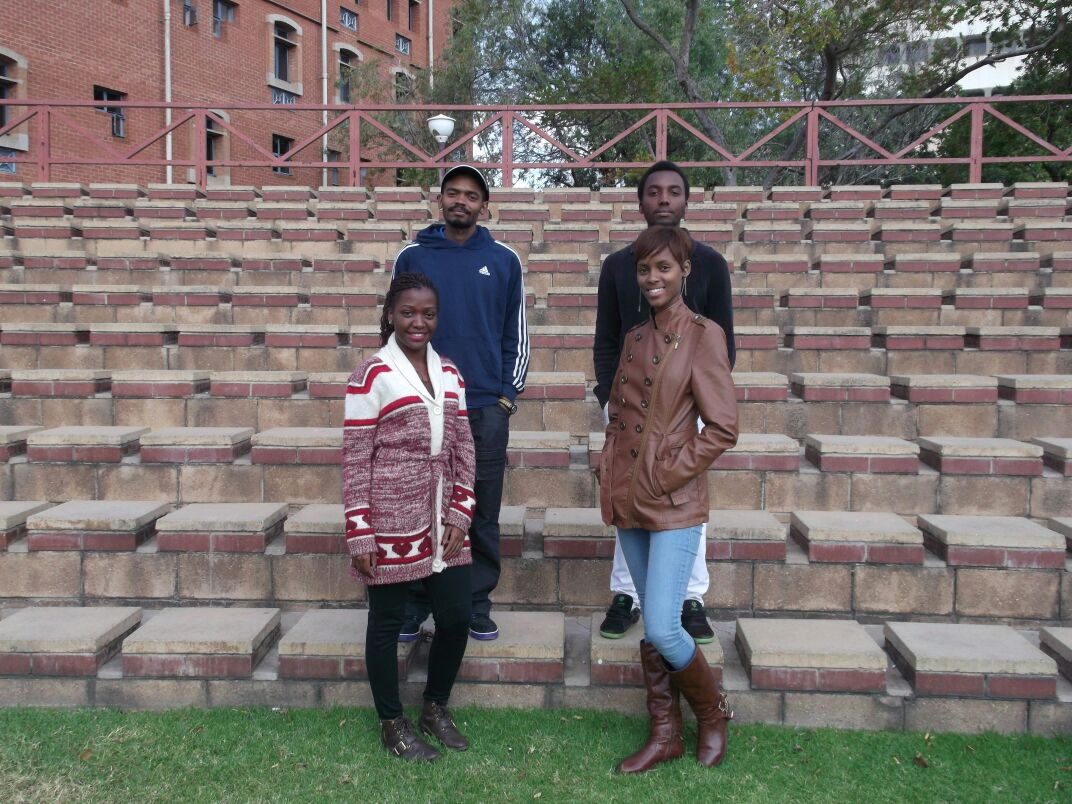
\includegraphics[width=\textwidth]{images/GroupPhoto}
\section{The Team}
\subsection{Mpho Baloyi}
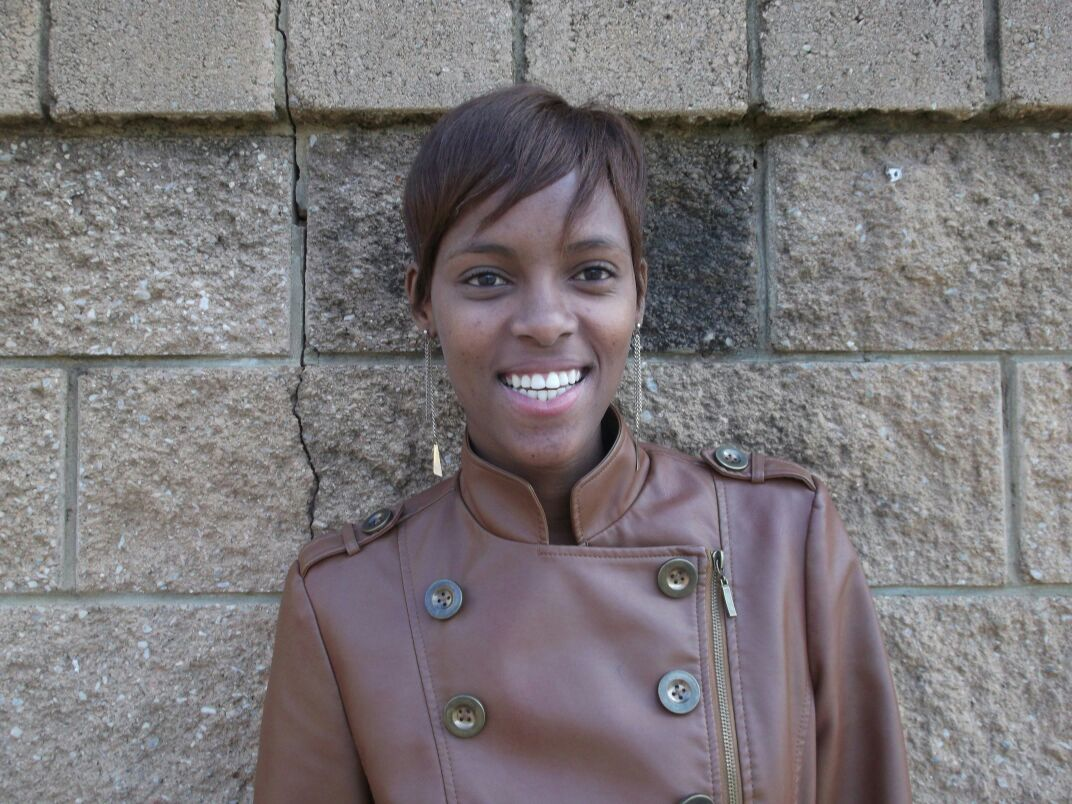
\includegraphics[width=\textwidth]{images/Mpho}
\subsubsection{Interests}
\begin{itemize}
\item Keeping abreast with new technologies
\item Learning and using new technologies to solve problems
\item Reading up and doing research on new and old concepts in computer science
\item Solving riddles and puzzles
\item Helping people through ICT
\end{itemize}
\subsubsection{Technical Skills}
\begin{itemize}
\item Solid programming skills in java,c++ and python
\item Fair amount of knowlegde in assembly programming
\item Web development with HTML,JAVASCRIPT,JQUERY,CSS,PHP,AJAX,ANGULARJS
\item Interaction Design
\item Database design with MySQL
\item Understanding of process development
\item Unit testing,mocking and dependency Injection
\end{itemize}
\subsubsection{Non-Technical Strengths}
\begin{itemize}
\item Excellent Communication skills
\item Patient
\item Creative approach to problem solving
\item Pay attention to detail
\item Excellent planning skills
\item Ability to grasp concepts quickly
\item Willness to learn new things
\item Ability to interpret and follow technical plans
\item Ability to collaborate and work efficiently with other people
\item Ability to work under pressure
\end{itemize}
\subsubsection{Relevant Past Experiences}
Work in the mini-project of the university of Pretoria taught me impoortant skills in software engineering such as unit testing,dependency injection,mocking and working with different technologies. I believe that these skills will be valuable to the development of this project as they apply in every area of software development.
\subsubsection{Reasons for wanting to do the project}
I want to do this project because it provides me with the opportunity to work with different kinds of technologies and devices and to learn new ways of collecting data.
\newpage
\subsection{Hlengekile Jita}
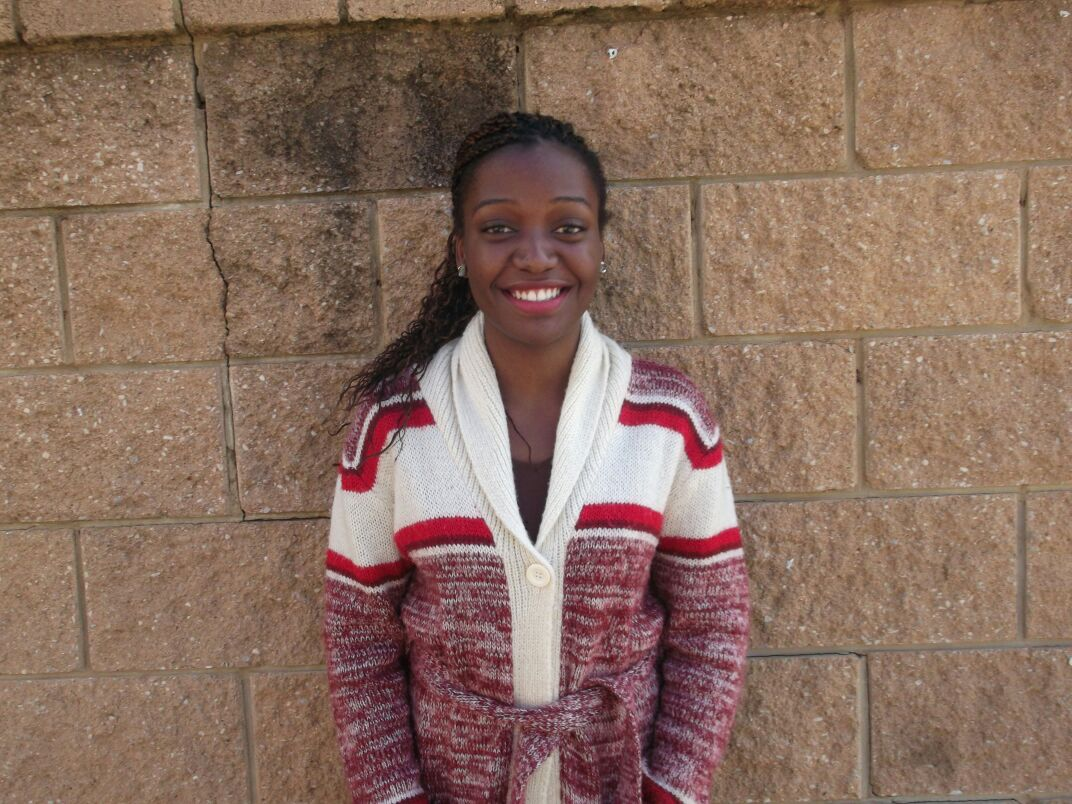
\includegraphics[width=\textwidth]{images/Hlengi}
\subsubsection{Interests}
\subsubsection{Technical Skills}
\begin{itemize}
\item Microsoft Office - Word, Excel, Access, PowerPoint
\item Programming - Java, C++, Python, Android
\item Database Design - MySQL
\item Web Development - XHTML, HTML5, CSS, JavaScript, PHP
\end{itemize}
\subsubsection{Non-Technical Strengths}
\begin{itemize}
\item Good leader
\item Excellent communication skills both verbal and written
\item Works well under pressure
\item Great at teamwork
\item Sociable character that gets along with people
\item Organized individual with meticulous planning skills
\item Determined
\end{itemize}
\subsubsection{Relevant Past Experiences}
\subsubsection{Reasons for wanting to do the project}
\newpage
\subsection{Moses Mayimela}
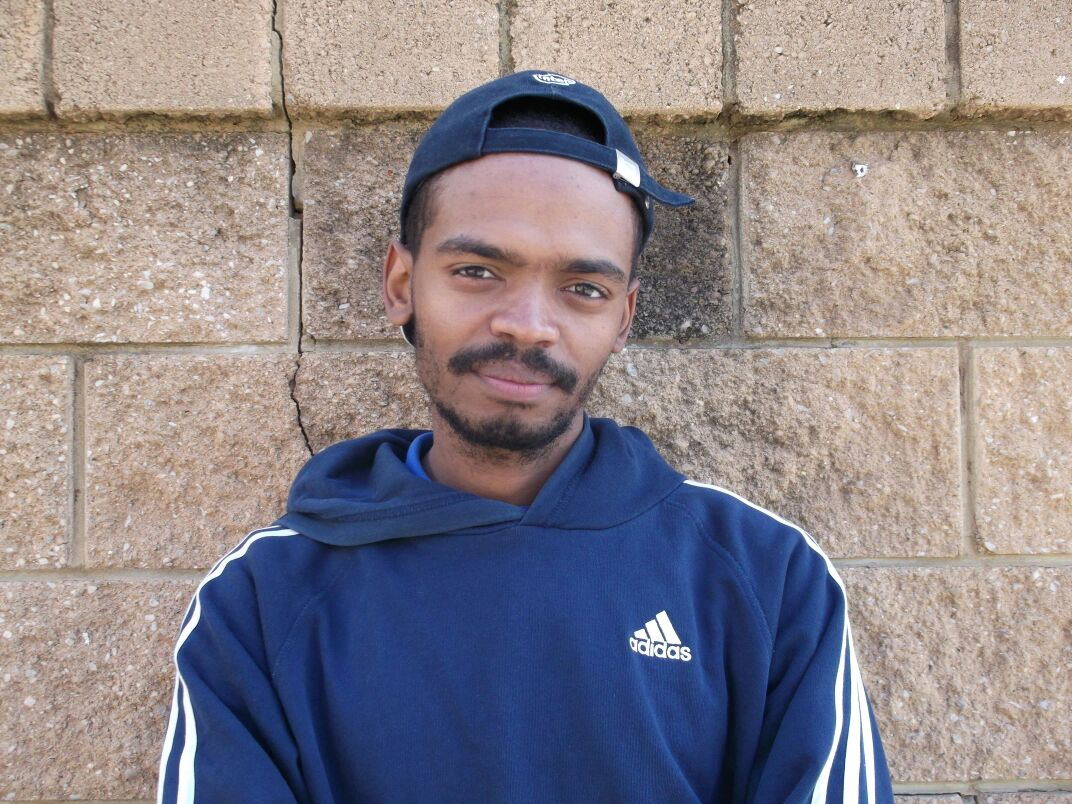
\includegraphics[width=\textwidth]{images/Moses}
\subsubsection{Interests}
\begin{itemize}
\item Keeping up to date with the latest technologies e.g Raspberry pi and Intel Edison.
\item Reading Tech reviews and comparisons on software and hardware systems such as BLE vs Classic bluetooth.
\item Taking part in hackerthons e.g Hack4Water.
\end{itemize}
\subsubsection{Technical Skills}
\begin{itemize}
\item Programming skills in:
\begin{enumerate}
\item Java.
\item C for embedded Systems (8 bit and 32 bit) and PC applications.
\item C++.
\item C\#.
\item Python.
\end{enumerate}
\item knowlegde in assembly programming for embedded (8 bit and 32 bit) and PC applications.
\item Web development with:\\
HTML,CSS, Javascript, NodeJS (Javascript framework),PHP and AJAX
\item Database design with MySQL,MSSQL and Postgresql.
\item Unit testing,mocking and dependency Injection
\item Familiar with GSM/3G Modules AT commands.
\item Experience with Linux servers.
\end{itemize}
\subsubsection{Non-Technical Strengths}
\begin{itemize}
\item I like working with people who love what they do.
\item I can lead a team and I also respect a leader.
\item I am always willing to learn and expand my horizons.
\item I am open minded to people's opinions.
\end{itemize}
\subsubsection{Relevant Past Experiences}
\begin{itemize}
\item Won, breakthrough developer award for 2015 in the MTN M2M (IoT) competition.\\
http://www.mind2machine.co.za \\
https://www.youtube.com/watch?v=HZlryrw1Ois.
\item 2nd place at the Hack4Water Hackathon in April 2016.\\
https://twitter.com/hashtag/hack4water
\end{itemize}
\subsubsection{Reasons for wanting to do the project}
This project will provide an opportunity for me to expand my knowledge in programming while providing a fully functional solution for the client. The technologies in this project will also help me learn better software standards. Through this project, I can personally learn how I can make myself better and improve my contribution in a way that matters when working with people.
\newpage
\subsection{Themba Mbhele}
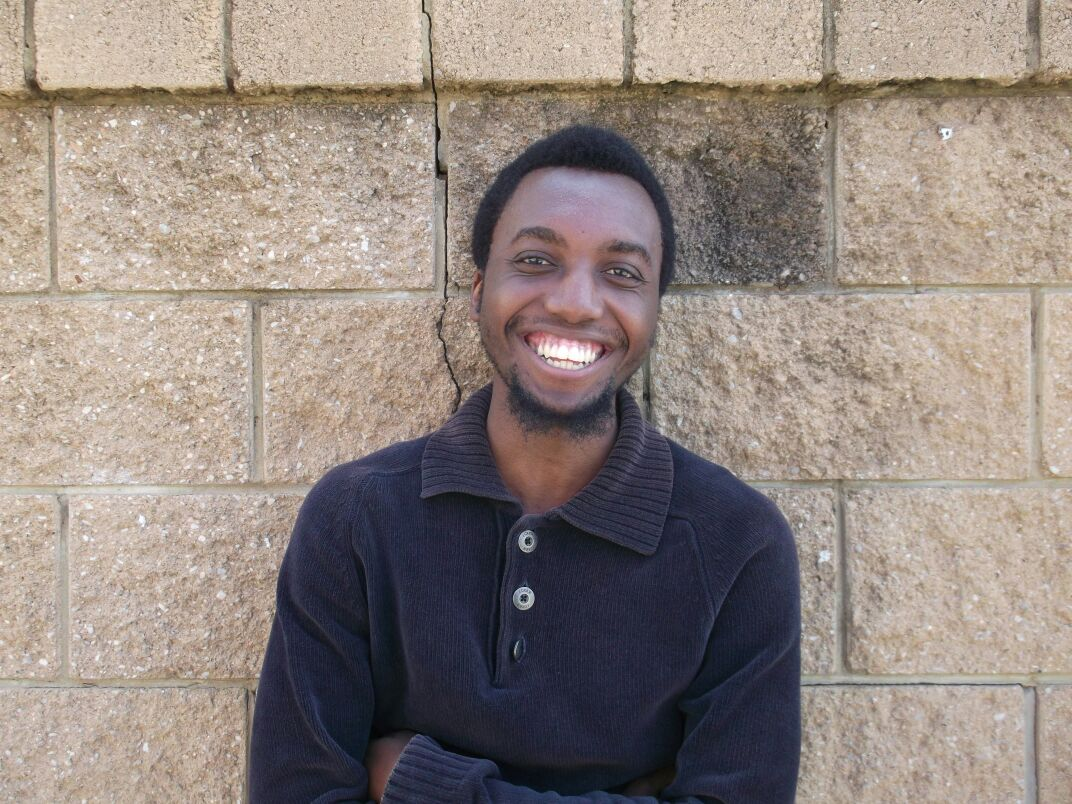
\includegraphics[width=\textwidth]{images/Themba}
\\subsubsection{Interests}
\begin{itemize}
    \item Gaming
    \item Artificial Intelligence
    \item Keeping up with the new developments in the Computer Science field
    \item Participating in IT challenges e.g Standard Bank IT Challenge
\end{itemize}
\subsubsection{Technical Skills}
\begin{itemize}
    \item Strong programming skills in C++ and Java
    \item Linux 64-bit assembler knowledge
    \item Unit testing, mocking, and dependency injection
    \item Web Dev - HTML5, CSS, WebGL, JavaScript, PHP
\end{itemize}
\subsubsection{Non-Technical Strengths}
\begin{itemize}
    \item Excellent time management skills
    \item I am a Dedicated student who will in the necessary effort to make a success of any projects that I am a part of.
    \item I am a Team player
\end{itemize}
\subsubsection{Reasons for wanting to do the project}
I believe that performance analysis is key not only to businesses, but also on a personal level. I want to be a part of this project so that I can learn what are the key performance measures that determine how optimal an 
individual or team is so that I may know which techniques or tactics should be used to improve efficiency.
\newpage
\section{Project Execution}
\subsection{Development Methodology}
For this project, there are three main development aspects, first programming the particle that logs data to the server, then the server which processes the data by performing mathematical analysis and finally the user interface provided by the web app where the processed data is displayed and the client is able to view the information.\\
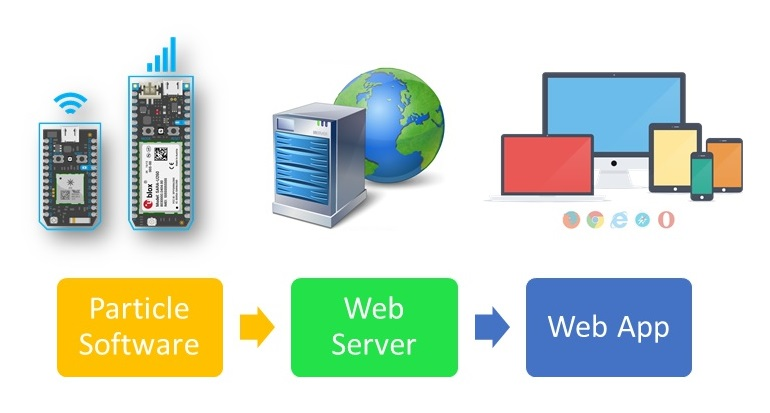
\includegraphics[width=\textwidth]{pcDevMeth.jpg}

On the first level, that is programming the particle, we would need to read data specific to power consumption and log this data to the server. This data includes data such as voltage and current. This information could be gathered using CT sensors connected to the electronic device. Once this data is logged to the server then it can be stored in a database so that at a later stage when a client makes a request using HTTPS the data can be retrieved and the necessary calculations can be performed and the server is able to respond appropriately. \\

Based on the above, we have decided to adopt an Agile Development Methodology and more specifically, Extreme Programming. Using this methodology we are able to incrementally build the software system using sprints where specific functionality is completed. We would like to continuously deliver high quality software. This would mean work very closely with the client, B{\"u}hler, and more specifically the project owner, Mr. Hanrich Potgieter. As we work together we will be able to identify numerous use cases that will become the focus of the sprints, the development team will complete. \\

Extreme Programming practices focus on having a continuous process, a shared understanding and giving feedback. These principles are important to our project because as previously mentioned, we would like our client to be satisfied hence we need to make sure that we have a proper understanding of their needs and provide them with working progress at regular intervals for their feedback. The practices that are key are:
\begin{itemize}
\item Planning
\item Test-Driven Development
\item Continuous Integration
\item Small Releases
\end{itemize}
The system will thus have to demonstrate working functionality at the end of each sprint and incrementally grow to its best form as it gains aspects of functionality. We will follow a development process of planning, design, implementation and testing at every sprint. In this way, because as the project progresses, development processes are completed as a whole, we only have to revisit completed aspects of the system if we have ways to modify and improve on it and not to make corrections because of faults.\\

In addition to this development process, other aspects of Extreme Programming that will add great value to the development of this power monitoring solution is:
\begin{itemize}
\item Pair programming, in this way code is continuously reviewed by the team.
\item Simple Design, in this way every member of the team is able to learn as we go and develop a rounded understanding of the system enabling the production of better software.
\item Sustainable pace, in this way we are able to produce our best work at all times, instead of trying to rapidly produce software that fails.
\end{itemize}
Our starting point will be the collection of data using the particle, and as we work with our client and identify units of functionality we begin the work on the server and interface which will be done simultaneously so that each unit can be put to user testing as the project progresses.
\subsection{Communication With Client}
To keep the clients informed we are going to use the following means of communication
\subsubsection{email}
\begin{itemize}
\item To inform the client of our progress
\item To address any issues or concerns that they client may have
\item To acquire information from the client
\item To require any resources that the client has to offer for their project,..
\end{itemize}

\subsubsection{Phone calls}
 This will only be used to address very urgent matters if they arise during the course of the project development 
 however this will only be done with permission from the client and during business hours.
 
\subsubsection{Regular Meetings}	 
These will take place depending on the clients availiability and willness.
We may discuss the progress of the project,to address any concerns,etc.

\subsubsection{GIT}

Access to our git repository will be provided to the client,so the client can be able to monitor
our progress and have access to the project material.

We are also open to any means of communicatiuon that the client may prefer or suggest.

\subsection{Technical Challenges}
\subsubsection{Collecting the readings}
The sensors or hardware that will be used to collect the physical readings have not been outlined and thus the challenge is how these values will be captured from the operating machinery.\\ \\
The solution:\\ 
Since the boards (photon and electron) have GPIOs, these can be used to interface with the various sensors that will capture the readings such as voltage and current. To measure current, a Current transformer, for example can be used to capture the operating current of a machine.\\
\\
To measure voltage, a step down transformer can be used to step down the voltage of the line connected in parallel to the operating machine. once the voltage has been stepped down to a level that the boards can tolerate i.e the max voltage would be 3.3V logic since the boards can operate at 3.3V VCC, then the signal can be fed to the analog pins of either the photon or the electron board.
\\ \\
These values, voltage and current are essential for the computation of other values such as power, e.g P=VI. 

\subsubsection{Connecting the photon to a local router}
The electron has a direct connection to the internet through the SARA-U260 module. The photon board, however needs a mobile device to get internet connection and thus thus the challenge will be to eliminate the need for a cellphone for the internet connection.\\ \\
The solution:\\
The approach to follow is to use a device that can connect more than one device to the internet e.g a wifi router. The router can provide all the photon boards with a connection to the internet. 
\subsection{Technologies}
This section will list the technologies that will be used to implement the system.\\
To implement the back-end of the system, the following technologies will be used:
\begin{itemize}
    \item NodeJS will be used to implement the server.
    \item MongoDB will be used to store the data that will be collected.
    \item C++ will be used to program the hardware
\end{itemize}
To implement the front-end of the system, the following technologies will be used:
\begin{itemize}
    \item AngularJS will be used for the web front-end.
\end{itemize}

\end{document}
